% document type
\documentclass[12pt]{article}

% packages
\usepackage[total={170mm,230mm}]{geometry}
\usepackage[utf8]{inputenc}
\usepackage[T1]{fontenc}
\usepackage[russian]{babel}
\usepackage{graphicx}
\usepackage{amssymb}
\usepackage{amsfonts}
\usepackage{amsmath}
\usepackage{amsthm}
\usepackage{physics}
\usepackage{nicefrac}
\usepackage{cancel}
\usepackage{hyperref}
\usepackage{cmap}

\title{Эффект Зеемана}
\author{Козлов Александр \and Краснощёкова Дарья}

\begin{document}
	%!TEX root = ../diode.tex
\begin{titlepage}
	\begin{center}
	% \vspace{-3em}
	{\small\textsc{Нижегородский государственный университет имени Н.\,И. Лобачевского}}
	\vskip 2pt \hrule \vskip 3pt
	{\small\textsc{Высшая школа общей и прикладной физики}}

	\vfill


	{{\large Отчет по лабораторной работе}\vskip 12 pt {\Large \bfseries Эффект Зеемана}}

		
	\vspace{2cm}
	{\large Работу выполнили студенты \\[0.5em]{\Large \bfseries Краснощёкова Дарья, Козлов Александр}}

	\end{center}

	\vfill

	\begin{center}
	{Нижний Новгород, \today}
	\end{center}
\end{titlepage}

	\tableofcontents
	\newpage

	\section{Расчёт расщепления рекомендуемых к наблюдению спектральных линий}
	\subsection*{$N=1,\:\lambda = 585.25\ \text{нм}$}
	Переход $J \rightarrow J+1$	осуществляется между комбинирующими уровнями $E_1\qty(J_1 = 0,\: L_1 = 0,\: S_1 = 0)$ и $E_2\qty(J_2 = 1,\: L_2 = 1,\: S_2 = 0)$. По формуле 
	\begin{equation}
	 	g = 1 + \dfrac{J(J+1) + S(S+1) - L(L+1)}{2J(J+1)}
	\end{equation}
	находим факторы Ланде $g_1 = ?,\: g_2 = 1$. Переходы, на которых возможно получение зеемановских компонент, показаны стрелками на рисунке \ref{fig:figure1}.
	\begin{figure}[htbp]
		\centering
		
\includegraphics[width=1\linewidth]{../images/1.png}
		\caption{Излучательные переходы, разрешённые правилами отбора для спектральной линии $\lambda = 585.25\ \text{нм}$.}
		\label{fig:figure1}
	\end{figure}
	Подставив в предложенные в методичке формулы входные данные, получаем расчёт расщепления для рассматриваемого пример. Результаты этого расчёта отражены в таблице \ref{table:1}.
	\begin{table}[h!]
		\centering
		\begin{tabular}{|c c c c c c|} 
 			\hline
 			$M_1$ & $M_2$ & $\Delta \omega_{M_1, M_2} \cdot \hbar / (\mu_0 H)$ & $I_{\perp}$ & $I_{\|}$ & Тип \\ [0.5ex] 
 			\hline
 			0 & -1 & 1 & $1/2$ & 1 & $\sigma$ \\
 			0 & 0 & 0 & $1$ & 0 & $\pi$ \\
 			0 & 1 & -1 & $1/2$ & 1 & $\sigma$ \\
 			\hline
		\end{tabular}
		\caption{Расщепление для спектральной линии $\lambda = 585.25\ \text{нм}$.}
		\label{table:1}
	\end{table}

	\subsection*{$N=3,\:\lambda = 594.48\ \text{нм}$}
	Переход $J \rightarrow J$	осуществляется между комбинирующими уровнями $E_1\qty(J_1 = 2,\: L_1 = 1,\: S_1 = 1)$ и $E_2\qty(J_2 = 2,\: L_2 = 1,\: S_2 = 1)$. Факторы Ланде $g_1 = 3/2,\: g_2 = 3/2$. Расщепление расчитано в таблице \ref{table:2}.
	\begin{table}[h!]
		\centering
		\begin{tabular}{|c c c c c c|} 
 			\hline
 			$M_1$ & $M_2$ & $\Delta \omega_{M_1, M_2} \cdot \hbar / (\mu_0 H)$ & $I_{\perp}$ & $I_{\|}$ & Тип \\ [0.5ex] 
 			\hline
 			-2 & -2 & 0 & 4 & 0 & $\pi$ \\
 			-2 & -1 & $-3/2$ & 1 & 2 & $\sigma$ \\
 			-1 & -2 & $3/2$ & 1 & 2 & $\sigma$ \\
 			-1 & -1 & $0$ & 1 & 0 & $\pi$ \\
 			-1 & 0 & $-3/2$ & $3/2$ & 3 & $\sigma$ \\
 			0 & -1 & $3/2$ & $3/2$ & 3 & $\sigma$ \\
 			0 & 0 & $0$ & $0$ & 0 & $\pi$ \\
 			0 & 1 & $-3/2$ & $3/2$ & 3 & $\sigma$ \\
 			1 & 0 & $-3/2$ & $3/2$ & 3 & $\sigma$ \\
 			1 & 1 & $0$ & $1$ & 0 & $\pi$ \\
 			1 & 2 & $-3/2$ & $1$ & 2 & $\sigma$ \\
 			2 & 1 & $3/2$ & $1$ & 2 & $\sigma$ \\
 			2 & 2 & 0 & 4 & 0 & $\pi$ \\
 			\hline
		\end{tabular}
		\caption{Расщепление для спектральной линии $\lambda = 594.48\ \text{нм}$.}
		\label{table:2}
	\end{table}

	\subsection*{$N=6,\:\lambda = 607.4\ \text{нм}$}
	Переход $J \rightarrow J+1$	осуществляется между комбинирующими уровнями $E_1\qty(J_1 = 0,\: L_1 = 1,\: S_1 = 1)$ и $E_2\qty(J_2 = 1,\: L_2 = 1,\: S_2 = 1)$. Факторы Ланде $g_1 = ?,\: g_2 = 3/2$. Расщепление рассчитано в таблице \ref{table:3}.
	\begin{table}[h!]
		\centering
		\begin{tabular}{|c c c c c c|} 
 			\hline
 			$M_1$ & $M_2$ & $\Delta \omega_{M_1, M_2} \cdot \hbar / (\mu_0 H)$ & $I_{\perp}$ & $I_{\|}$ & Тип \\ [0.5ex] 
 			\hline
 			0 & -1 & $3/2$ & $1/2$ & 1 & $\sigma$ \\
 			0 & 0 & 0 & $1$ & 0 & $\pi$ \\
 			0 & 1 & $-3/2$ & $1/2$ & 1 & $\sigma$ \\
 			\hline
		\end{tabular}
		\caption{Расщепление для спектральной линии $\lambda = 607.4\ \text{нм}$.}
		\label{table:3}
	\end{table}

	\subsection*{$N=14,\:\lambda =638.3\ \text{нм}$}
	Переход $J \rightarrow J$	осуществляется между комбинирующими уровнями $E_1\qty(J_1 = 1,\: L_1 = 2,\: S_1 = 1)$ и $E_2\qty(J_2 = 1,\: L_2 = 1,\: S_2 = 1)$. Факторы Ланде $g_1 = 1/2,\: g_2 = 3/2$. Расщепление расчитано в таблице \ref{table:4}.
	\begin{table}[h!]
		\centering
		\begin{tabular}{|c c c c c c|} 
 			\hline
 			$M_1$ & $M_2$ & $\Delta \omega_{M_1, M_2} \cdot \hbar / (\mu_0 H)$ & $I_{\perp}$ & $I_{\|}$ & Тип \\ [0.5ex] 
 			\hline
 			-1 & -1 & $1$ & $1$ & $0$ & $\pi$ \\
 			-1 & 0 & $-1/2$ & $1/2$ & $1$ & $\sigma$ \\
 			0 & -1 & $3/2$ & $1/2$ & $1$ & $\sigma$ \\
 			0 & 0 & $0$ & $0$ & $0$ & $\pi$ \\
 			0 & 1 & $-3/2$ & $1/2$ & $1$ & $\sigma$ \\
 			1 & 0 & $1/2$ & $1/2$ & $1$ & $\sigma$ \\
 			1 & 1 & $-1$ & $1$ & $0$ & $\sigma$ \\
 			\hline
		\end{tabular}
		\caption{Расщепление для спектральной линии $\lambda = 638.3\ \text{нм}$.}
		\label{table:4}
	\end{table}

	\section{Немного про экспериментальную установку}
	Мы изучали эффект Зеемана на примере спектра излучения неона с помощью интерферометра Фабри\---Перо (ИФП). ИФП является многолучевым интерферометром высокой разрешающей способности. Он состоит из двух прозрачных клиновидных пластин, внутренние поверхности которых ограничивают плоскопараллельный слой воздуха. На эти поверхности нанесено диэлектрической покрытие, обеспечивающее энергетический коэффициент отражения $\rho$, близкий к единице.
	\par Луч, вошедший в интерферометр и многократно отразившийся от зеркальных поверхностей, образует ряд проходящих параллельных лучей с постоянной разностью хода
	\begin{equation}
		\Delta = 2h\cos{\Psi},
	\end{equation}
	где через $h$ обозначена толщина воздушного слоя, а $\Psi \ll 1$ обозначает угол падения света в зазор.
	\par Объектив, установленный после ИФП, формирует линии равного наклона, представляющие собой систему концентрических колец. Угловые размеры колец $\Psi_i$ определяются из условия интерференционного максимума
	\begin{equation}
		2h\cos{\Psi_i} = m_i \lambda = m_0 \lambda \cos{\Psi_i},
	\end{equation} 
	где $m_i$ \---- это порядок интерференции (большое целое число, так как размеры воздушного зазора макроскопичны), а $m_0 = 2h / \lambda$ \---- максимальный порядок интерференции, который отвечает $\Psi_i=0$. Индекс $i$ растёт от центра интерференционной картины и обозначает номер кольца.
	\par Диаметр колец Фабри\---Перо определяется формулой
	\begin{equation}
		d^2_i = \dfrac{4f^2\lambda(m_0-m_i)}{h},
	\end{equation}
	где $f$ \---- фокусное расстояние объектива. Можно ввести дробную долю порядка интерференции $\varepsilon_\lambda$, которая определяется следующим образом
	\begin{equation}
		m_0-m_i = i - 1 + \varepsilon_\lambda.
	\end{equation}
	\par Характерными особенностями ИФП как спектрального прибора является высокая разрешающая способность
	\begin{equation}\label{eq:6}
		R = \dfrac{m_0 \pi \sqrt{\rho}}{1-\rho}
	\end{equation}
	и малая дисперсионная область (интервал длин волн, где можно наблюдать интерференционную картину без наложения соседних порядков)
	\begin{equation}
		\Delta \lambda = \dfrac{\lambda^2}{2h\cos{\Psi}}.
	\end{equation}
	Это приводит к тому, что надо использовать спектрограф. ИФП устанавливается так, чтобы плоскость локализации колец совместилась с плоскостью щели спектрографа, которая вырезает из колец узкую вертикальную полоску. Таким образом, спектрограф разлагает свет в спектр в горизонтальной плоскости, а ИФП \---- вдоль вертикальной входной щели спектрографа.

	\section{Наблюдение нормального эффекта Зеемана на примере линии 585.25 нм}
	\subsection{Исследование характера поляризации линий в поперечном эффекте}
	Пронаблюдали характер поляризации компонент в поперечном эффекте (продольный эффект не мог быть нами наблюдаем по причине негодности установки). Убедились, что при наблюдении поперечного эффекта $\sigma$ и $\pi$ линии поляризованы линейно в перпендикулярных друг другу плоскостях.

	\subsection{Измерение расщепления линий в поперечном эффекте и определение удельного заряда электрона}
	При магнитном поле $H = 6600\ \text{Э}$ измерили расщепление в поперечном эффекте. Для наглядности приведём смысл используемых ниже обозначений на рисунке \ref{fig:figure2}.
	\begin{figure}[htbp]
		\centering
		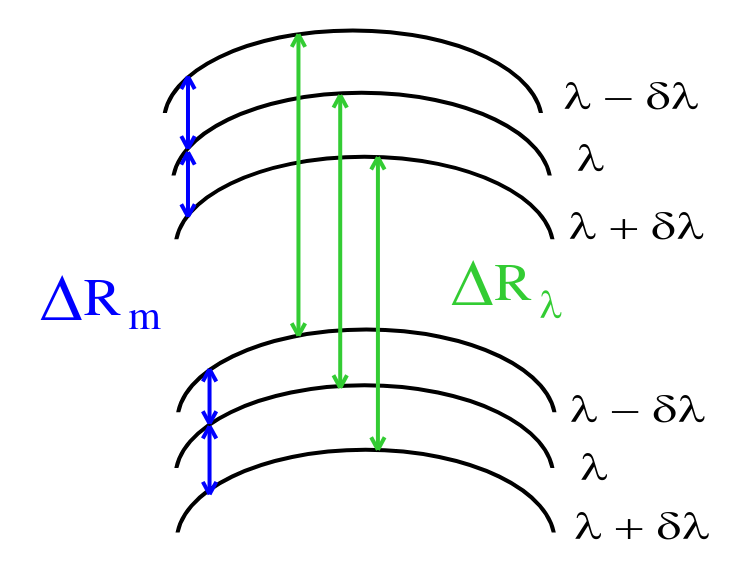
\includegraphics[width=1\linewidth]{../images/2.png}
		\caption{Вид двух соседних колец при расщеплении спектральной линии в магнитном поле. $\Delta R_m$ \---- разность радиусов колец одного порядка интерференции, образованных излучением разных длин волн $(\lambda-\Delta\lambda,\:\lambda,\:\lambda+\Delta\lambda)$. $\Delta R_\lambda$ \---- разность радиусов колец разных порядков интерференции, образованных излучением одной длины волны.}
		\label{fig:figure2}
	\end{figure}
	Результаты измерений занесли в таблицу \ref{table:5}.
	\begin{table}[h!]
		\centering
		\begin{tabular}{|c c c c | c |} 
 			\hline
 			$\Delta R_{m_1}$ & $\Delta R_{m_2}$ & $\Delta R_{m_3}$ & $\Delta R_{m_4}$ & $\expval{\Delta R_m}$ \\
 			\hline
 			10 & 7 & 8 & 10 & $8.75\pm1.30$ \\
 			\hline\hline
 			$\Delta R_{\lambda_1}$ & $\Delta R_{\lambda_2}$ & $\Delta R_{\lambda_3}$ & \---- & $\expval{\Delta R_\lambda}$ \\
 			\hline
 			25& 23& 26& \---- & $24.67\pm1.25$\\
 			\hline
		\end{tabular}
		\caption{Результаты измерений расщепления для спектральной линии $\lambda = 585.25\ \text{нм}$.}
		\label{table:5}
	\end{table}
	Для расщепления была заявлена в методичке следующая формула:
	\begin{equation}
		\delta\lambda = \dfrac{\lambda^2}{2h}\dfrac{\expval{\Delta R_m}}{\expval{\Delta R_\lambda}}.
	\end{equation}
	По ней и будет вестись расчёт. Заметим, что $h = 4\ \text{мм}$. Подставив, получаем
	\begin{equation}
		\delta\lambda = (1.52\pm0.30 )\cdot 10^{-9}\ \text{см}.
	\end{equation}
	\par Теперь вычислим удельный заряд электрона. Для этого учтём, что при наложении магнитного поля наблюдаемые в поперечном эффекте частоты $\omega_{1,2} = \omega_0 \pm \Omega$. Откуда получаем формулу для вычисления циклотронной частоты
	\begin{equation}
		\Omega = \delta\omega.
	\end{equation}
	Разницу частот можно вычислить, как
	\begin{equation}
		\delta\omega = 2\pi c\qty(\dfrac{1}{\lambda} - \dfrac{1}{\lambda+\delta\lambda}) = 2\pi c \dfrac{\delta\lambda}{\lambda(\lambda+\delta\lambda)}
	\end{equation}
	А погрешность можно сосчитать, как
	\begin{equation}
		\dd{\delta\omega} = 2\pi c \dfrac{\dd{\delta\lambda}}{(\lambda+\delta\lambda)^2}.
	\end{equation}
	Тогда 
	\begin{equation}
		\Omega = \delta\omega = (8.36\pm1.65)\cdot10^{10}\ \text{с}{}^{-1}.
	\end{equation}
	С другой стороны, по определению циклотронная частота 
	\begin{equation}
		\Omega = \dfrac{e}{m} \dfrac{H}{c}.
	\end{equation}
	Значит, удельный заряд электрона может быть вычислен
	\begin{equation}
		\dfrac{e}{m} = (3.80\pm0.75)\cdot10^{17}\ \text{в единицах СГС}.
	\end{equation}
	Отметим, что табличное значение данной величины в единицах СГС составляет $5.27\cdot10^{17}$.

	\subsection{Оценка разрешающей способности ИФП и её сопоставление с расчётной величиной}
	Прежде всего произведём расчёт разрешающей способность по формуле \ref{eq:6}, с учётом того, что $m_0 = 2h/\lambda$. Для этого потребуется численные значения энергетического коэффициента отражения $\rho$ и ширины воздушного зазора $h$. В лаборатории мы узнали, что $\rho = 0.89$, a $h = 4\ \text{мм}$. Тогда не составляет труда получить, что $R_{theor} = 3.68 \cdot 10^5$. Это расчётная величина, с ней будем сравнивать результаты измерений.
	\par Наблюдаемую разрешающую способность будем понимать, как отношение
	\begin{equation}
		R_{exp} = \dfrac{\omega}{\delta \omega}.
	\end{equation}
	Если учесть, что $\omega = 2\pi c / \lambda$ и $\delta \omega = H\mu_0 / \hbar$, то получим при поле 3675 Э, при котором линии сливаются, следующий результат:
	\begin{equation}
		R_{exp} = \dfrac{2\pi c \hbar}{H \mu_0 \lambda} \approx 9.96 \cdot 10^4.
	\end{equation}
	Таким образом реальная разрешающая способность в $3.69$ раз меньше, чем расчётная. Тем не менее это величины одного порядка. Расхождение можно объяснить тем, что спектральная линия лампы имеет небольшую, но конечную ширину вследствие взаимодействия атомов неона со стенками и друг с другом, поэтому точность измерений не очень высока.

	\section{Изучение аномального эффекта Зеемана в квазинормальном случае на примере линии 607.4 нм}
	\subsection{Исследование характера компонент в поперечном эффекте}
	Исследовали характер компонент в поперечном эффекте, определили, что каждая линия поляризована линейно, и то, что средние линии поляризованы в плоскостях, перпендикулярных плоскостям поляризации крайних линий. Что отвечает теории из методички. Вид наблюдаемой картины изображён на рисунке \ref{fig:figure3}.
	\begin{figure}[htbp]
	 	\centering
	 	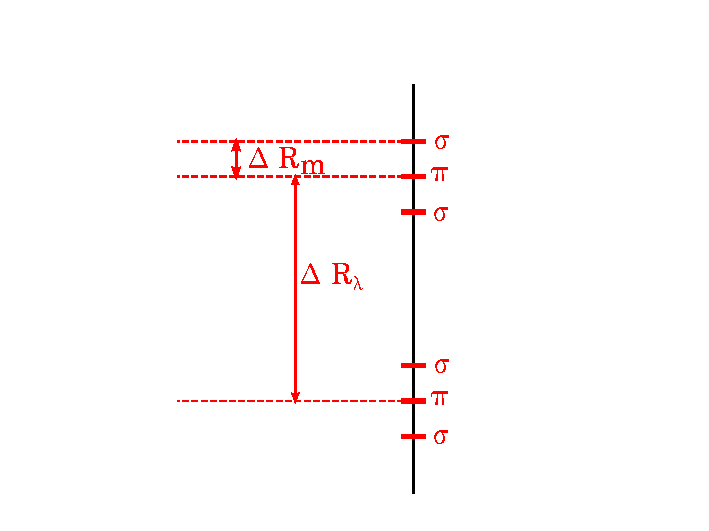
\includegraphics[width=\linewidth]{../images/3}
	 	\caption{Картина расщепления для поперечного эффекта в линии 607.4 нм.}
	 	\label{fig:figure3}
	 \end{figure}

	 \subsection{Измерение расщепления и определение факторов Ланде}
	 Результаты измерений расщепления при поле в 5406 Э приведены в таблице \ref{table:6}.
	 \begin{table}[h!]
		\centering
		\begin{tabular}{|c c c c | c |} 
 			\hline
 			$\Delta R_{m_1}$ & $\Delta R_{m_2}$ & $\Delta R_{m_3}$ & $\Delta R_{m_4}$ & $\expval{\Delta R_m}$ \\
 			\hline
 			6 & 5 & 7 & 8 & $6.5\pm1.12$ \\
 			\hline\hline
 			$\Delta R_{\lambda_1}$ & $\Delta R_{\lambda_2}$ & $\Delta R_{\lambda_3}$ & \---- & $\expval{\Delta R_\lambda}$ \\
 			\hline
 			31& 28& 27& \---- & $28.67\pm1.70$\\
 			\hline
		\end{tabular}
		\caption{Результаты измерений расщепления для спектральной линии 607.4 нм при магнитном поле 5406 Э.}
		\label{table:6}
	\end{table}
	Откуда по уже известной методике мы восстанавливаем 
	\begin{equation}
		\delta \lambda = (1.05\pm0.24)\cdot 10^{-9}\ \text{см}.
	\end{equation}
	А оттуда находим и 
	\begin{equation}
		\delta \omega = (5.36 \pm 1.23)\cdot10^{10}\ \text{рад с}{}^{-1}.
	\end{equation}
	\par Теперь определим факторы Ланде. При это можно не брать в рассмотрение фактор для исходного состояния, так как всё равно $M_1 = 0$. Тогда теоретический расчёт в LS\---приближении даёт
	\begin{equation}
		g_2 = \dfrac{3}{2}.
	\end{equation}
	Посмотрим, что мы получаем в эксперименте. Тут надо пользоваться формулой
	\begin{equation}
		\delta\omega = \abs{g_2 M_2} \dfrac{\mu_0H}{\hbar}\Longrightarrow \abs{g_2} = \dfrac{\delta\omega\hbar}{\abs{M_2}\mu_0H}.
	\end{equation}
	Кладём $\abs{M_2} = 1$ и получаем %тут ещё поделил на два пи, чтобы нормальные ответы были, хз что здесь творится!
	\begin{equation}
		\abs{g_2} = 1.13\pm0.25,
	\end{equation}
	что достаточно близко к предсказанному грубой теорией значению.

	\section{Изучение аномального эффекта Зеемана на примере линии 638.3 нм}
	Из теоретических расчетов в LS\---приближении при расщеплении должно получиться 6 линий, соответствующих изменению безразмерной частоты $\pm1/2,\: \pm1,\: \pm3/2$. Однако, в эксперименте наблюдаются 2 линии с $\pi$\---поляризацией, которые дополнительно расщепляются на 4 линии с $\sigma$\---поляризацией, расположенные ближе, чем в теории. Таким образом, в одном порядке интерференции имеется 2 триплета, но из-за особенностей установки нам не удалось разрешить расщепленные $\sigma$\---компоненты.
	\par Результаты наблюдений расщепления представлены в таблице \ref{table:7}.
	\begin{table}[h!]
		\centering
		\begin{tabular}{|c c c c | c |} 
 			\hline
 			$\Delta R_{m_1}$ & $\Delta R_{m_2}$ & $\Delta R_{m_3}$ & $\Delta R_{m_4}$ & $\expval{\Delta R_m}$ \\
 			\hline
 			9 & 11 & \---- & \---- & $10\pm1$ \\
 			\hline\hline
 			$\Delta R_{\lambda_1}$ & $\Delta R_{\lambda_2}$ & $\Delta R_{\lambda_3}$ & \---- & $\expval{\Delta R_\lambda}$ \\
 			\hline
 			24& 25& \----& \---- & $25\pm1$\\
 			\hline
		\end{tabular}
		\caption{Результаты измерений расщепления для спектральной линии 638.3 нм при магнитном поле 6750 Э.}
		\label{table:7}
	\end{table}
	Вычисляем расщепление $\pi$\---компонент при магнитном поле 6750 Э
	\begin{equation}
		\delta\lambda = (1.84\pm0.26)\cdot10^{-9}\ \text{см}.
	\end{equation}
	Откуда получаем
	\begin{equation}
		\delta\omega = (8.53\pm1.19)\cdot10^{10}\ \text{рад с}{}^{-1}.
	\end{equation}
	Ещё надо найти разность факторов Ланде. В теории её модуль равен 1. Посмотрим, что мы имеем в эксперименте %опять эта хуйня с 2пи
	\begin{equation}
		\abs{g_1 - g_2} = \dfrac{\delta\omega\hbar}{H\mu_0} = 1.43\pm0.20.
	\end{equation}
\end{document}